\documentclass[11pt,a4paper]{article}

\usepackage[a4paper,margin=24mm]{geometry}
\usepackage{fontspec}
\usepackage{unicode-math}
\setmainfont{texgyretermes-regular.otf}[
  BoldFont=texgyretermes-bold.otf,
  ItalicFont=texgyretermes-italic.otf,
  BoldItalicFont=texgyretermes-bolditalic.otf]
\setsansfont{texgyreheros-regular.otf}[BoldFont=texgyreheros-bold.otf]
\setmonofont{lmmono10-regular.otf}[Scale=MatchLowercase]
\setmathfont{latinmodern-math.otf}
\setmathfont{latinmodern-math.otf}[version=bold,FakeBold=1.5]
\usepackage{microtype}
\usepackage{amsmath}
\usepackage{graphicx}
\usepackage{booktabs}
\usepackage{threeparttable}
\usepackage{array}
\usepackage{tabularx}
\usepackage{siunitx}
\usepackage{xcolor}
\usepackage{enumitem}
\usepackage[numbers,sort&compress]{natbib}
\usepackage[hidelinks]{hyperref}
\usepackage{caption}
\usepackage{subcaption}
\usepackage{placeins}

\graphicspath{{../../figures/}}
\captionsetup{font=small,labelfont=bf,labelsep=period,justification=justified,singlelinecheck=false}
\sisetup{round-mode=places,round-precision=3,detect-all}
\setlength{\parindent}{1.35em}
\setlength{\parskip}{0.20em}
\setlength{\emergencystretch}{2em}
\renewcommand{\arraystretch}{1.10}
\renewcommand{\baselinestretch}{1.06}
\newcommand{\SSCL}{\textsc{SSCL}}
\newcommand{\vect}[1]{\boldsymbol{#1}}

\title{Recovering Historical Chinese Incense Formulas under Source and Missingness Shift}
\author{Anonymous manuscript}
\date{}

\begin{document}
\maketitle

\begin{abstract}
Historical incense books transmit recipes through compilations that differ in vocabulary, ingredient frequency, and formula structure. We study whether ingredient relations learned from several work groups can recover hidden materials in an unseen work. The benchmark contains 91 family-unique formulas, 81 canonical aromatic materials, and six historical work groups. Models receive half of each formula and predict the remaining ingredients and composition. Nested leave-one-work-out evaluation selects hyperparameters inside each outer training fold. A directed conditional graph raised source-macro hidden-ingredient F1 from 0.378 for global frequency to 0.426. A source-stable conditional-lift extension reached 0.426 and improved five work groups with one tie against frequency; its difference from the direct graph was 0.0003 F1. EASE reached the highest weighted Jaccard, 0.473. Model ordering changed under abundance-biased, prefix, and unknown-fraction missingness. Nested logit calibration reduced source-macro Brier score from 0.0427 to 0.0340 and adaptive calibration error from 0.0579 to 0.0145. A chemical-similarity kernel covering 18 materials did not improve completion. The main transferable signal is conditional co-formulation, and its measured value depends on both source and observation process.
\end{abstract}

\noindent\textbf{Keywords:} graph-based set completion; computational heritage; historical recipes; domain shift; missing data; cheminformatics

\section{Introduction}

Historical smell research has developed methods for documenting odor objects, vocabularies, places, and sensory experiences \citep{bembibre2017_smell_heritage,lisena2022_odeuropa}. Chemical analysis can reconstruct a surviving residue when a physical sample remains \citep{paolin2026_historical_smells}. Incense books often present a harder case. A formula can survive as a title, a partial ingredient list, or a later compilation, with no material sample available for chromatography or sensory testing.

Computational olfaction maps molecular structure, spectra, or controlled mixtures to perceptual descriptors \citep{keller2017_dream,gutierrez2018_semantic,lee2023_pom,sisson2025_blends}. Inverse scent design optimizes modern mixtures against a requested odor profile \citep{aleixandre2024_scent_creation}. Historical formula recovery has a different input and target. The ingredients are natural materials with variable composition, the observations are incomplete recipe records, and the source documents carry distinct editorial and compositional conventions.

This study asks one question: which ingredient relations transfer when the target formula comes from a historical work excluded from training? We cast each formula as a sparse weighted set. The observed ingredients provide context, and the model ranks hidden materials and allocates the remaining mass. Each work group defines a source domain. The historical work is the evaluation unit because formulas in the same compilation share transmission history and terminology.

The study contributes a source-indexed benchmark and an evaluation protocol built around the target question. It compares global frequency, direct conditional co-occurrence, EASE, a SLIM-style item model, personalized graph diffusion, and a source-stable conditional-lift extension. It also tests four observation mechanisms and calibrates candidate probabilities inside the nested source folds. The useful signal lies in conditional co-formulation. The proposed source-stability penalty and the simpler directed graph differ by 0.0003 F1.

\section{Related Work}

\subsection{Olfactory data and inverse mixture design}

Molecular odor prediction uses physicochemical descriptors, learned molecular representations, and curated perceptual labels \citep{keller2017_dream,gutierrez2018_semantic,lee2023_pom,hamel2024_pyrfume}. Blend prediction adds nonlinear interactions between odorants \citep{sisson2025_blends,thomasdanguin2014_mixtures}. These models describe molecules or controlled mixtures. Incense ingredients such as agarwood, sandalwood, resins, and processed botanicals contain many compounds whose abundance changes with taxon, plant part, preparation, and combustion. Formula completion therefore uses chemistry as supporting material evidence; it has no direct chemical measurement of the target formula.

\subsection{Missing-label learning and recommendation}

Partial formula recovery is a multi-label problem with missing positive labels. Mixed-graph multi-label methods propagate information through instance and class dependencies \citep{wu2015mlmg,zhao2018_bayesian_multilabel}. Item-based recommender models provide strong small-data comparators. EASE estimates a dense zero-diagonal item matrix by ridge regression \citep{steck2019ease}; SLIM estimates a sparse nonnegative item matrix with elastic-net regularization \citep{ning2011slim}. Nearest-neighbour and low-rank recommendation test whether formula similarity or latent structure is sufficient \citep{cover1967_nearest_neighbor,cremonesi2010_topn}.

\subsection{Transfer and probability calibration}

Source-blocked evaluation follows the broader study of performance under distribution shift \citep{koh2021_wilds}. Cross-network transfer theory relates target error to both source performance and source-target graph discrepancy \citep{wu2023noniid}. Our corpus is too small to estimate a target graph before prediction, so the model measures heterogeneity among training-source conditional relations. Calibration is fitted on held-out source predictions. Temperature scaling supplies a one-parameter comparator \citep{guo2017_calibration}, and adaptive calibration error gives roughly equal-count probability groups \citep{nixon2019calibration}.

\section{Corpus and Prediction Task}

\subsection{Reference corpus}

The corpus was assembled from public-domain Chinese incense texts and public transcriptions. Each candidate record retained the work identifier, formula title, source span, locator, material mentions, quantities, and processing notes. Aromatic masses were converted to a common relative unit and closed to sum to one. Binders, liquids, and processing aids were stored separately. Records with unresolved aromatic quantities or uncertain formula boundaries were excluded. Canonicalization preserved the source expression and mapped accepted mentions to one of 81 material identifiers. Grade terms for agarwood remained distinct.

The resulting dataset contains 91 family-unique formulas from six work groups (Table~\ref{tab:corpus}). Formula size ranges from 2 to 17 materials, with mean 6.85 and median 6. Thirty materials occur once, and four occur in more than 40 formulas. One Huizhai formula has fewer than two in-vocabulary materials in its outer training fold and is excluded from completion metrics, leaving 90 evaluated formulas. All 91 records remain part of the released corpus.

\begin{table}[t]
\centering
\caption{Historical work groups in the reference corpus. Evaluation count is the number of formulas with at least two materials represented in the corresponding outer-fold training vocabulary.}
\label{tab:corpus}
\begin{threeparttable}
\begin{tabular}{lrr}
\toprule
Work group & Corpus formulas & Evaluated formulas \\
\midrule
Chen Xiangpu compilation & 38 & 38 \\
Xiangcheng compilation & 29 & 29 \\
Huizhai Xiangpu & 10 & 9 \\
Hong Xiangpu attribution & 6 & 6 \\
Liexiang Xinpu & 6 & 6 \\
Moe Xiaolu Xiangpu & 2 & 2 \\
\midrule
Total & 91 & 90 \\
\bottomrule
\end{tabular}
\end{threeparttable}
\end{table}

\subsection{Weighted set representation}

For formula $i$, $q_{ij}$ is the converted aromatic mass of material $j$, and $S_i$ is its support. The closed composition is
\begin{equation}
\vect{w}_i\in\Delta^{M-1},\qquad
w_{ij}=\frac{q_{ij}}{\sum_{k\in S_i}q_{ik}},\qquad
S_i=\{j:w_{ij}>0\}.
\label{eq:closure}
\end{equation}
The model receives an observed subset $O_i\subset S_i$ with its original mass fractions. It returns hidden-ingredient scores, a completed support, and a closed composition:
\begin{equation}
\mathcal{F}:\bigl(O_i,\{w_{ij}:j\in O_i\}\bigr)
\longmapsto \left(\{p_{ij}:j\notin O_i\},\widehat S_i,\widehat{\vect{w}}_i\right),
\qquad H_i=S_i\mathbin{\backslash}O_i.
\label{eq:task}
\end{equation}

\begin{table}[t]
\centering
\caption{Notation used in the model and evaluation. Every mathematical symbol in the first column is set in math mode.}
\label{tab:notation}
\small
\begin{tabularx}{\linewidth}{@{}lX@{}}
\toprule
\multicolumn{1}{c}{Symbol} & Meaning \\
\midrule
$i,j,a,b,d$ & Formula, candidate material, observed material, candidate material, and work indices \\
$S_i,O_i,H_i$ & Complete, observed, and hidden material sets for formula $i$ \\
$q_{ij},w_{ij}$ & Converted aromatic mass and closed mass fraction \\
$N_d,c_{ad},c_{abd}$ & Formula count, exposure count, and pair count within work $d$ \\
$\pi_b,\pi_{bd}$ & Global and work-specific prevalence of material $b$ \\
$\ell_{abd}$ & Conditional log-odds lift for edge $a\rightarrow b$ in work $d$ \\
$\mu_{ab},\sigma_{ab}$ & Weighted mean and standard deviation of source-specific lifts \\
$G_{ab},S_{ab}$ & Direct conditional and source-stable edge values \\
$p_{ij}$ & Candidate inclusion score or calibrated probability \\
$K_i,\widehat K_i$ & True and predicted total ingredient counts \\
$D,A_i$ & Number of outer work folds and repeated masks for formula $i$ \\
\bottomrule
\end{tabularx}
\end{table}

\subsection{Observation mechanisms}

The primary task retains half of the in-vocabulary materials. If $K_i=|S_i|$ and $f$ is the requested fraction, the observed count is
\begin{equation}
r(K_i,f)=\min\{K_i-1,\max[1,\operatorname{round}(fK_i)]\}.
\label{eq:maskcount}
\end{equation}
Five deterministic seeds select uniform subsets at $f=0.50$. Secondary tests use $f\in\{0.25,0.50,0.75\}$ and four mechanisms: uniform retention, abundance-biased retention, a prefix of the source list, and uniform retention with the decoder unaware of $f$. Hash-based seeding makes every mask reproducible.

\section{Models}

\subsection{Global and direct conditional baselines}

Let $X\in\{0,1\}^{N\times M}$ be the training presence matrix. With $c_b=\sum_i X_{ib}$, the smoothed global prevalence is
\begin{equation}
\pi_b=\frac{c_b+\tfrac12}{N+1}.
\label{eq:globalprev}
\end{equation}
The frequency baseline ranks candidates by $\pi_b$. For the directed graph, $c_a$ counts formulas containing $a$, and $c_{ab}$ counts formulas containing both $a$ and $b$. Its edge is
\begin{equation}
G_{ab}=\frac{c_{ab}+\alpha\pi_b}{c_a+\alpha},\qquad G_{aa}=1.
\label{eq:directgraph}
\end{equation}
This estimator is asymmetric because the denominators depend on the source material.

\subsection{Source-stable conditional lift}

\SSCL{} estimates the relation separately in each training work. Work prevalence shrinks toward the global prevalence:
\begin{equation}
\pi_{bd}=\frac{c_{bd}+\kappa\pi_b}{N_d+\kappa}.
\label{eq:sourceprev}
\end{equation}
For edge $a\rightarrow b$, the smoothed conditional probability is also the posterior mean under a beta prior:
\begin{align}
\theta_{abd}\mid\mathcal{D}
&\sim \operatorname{Beta}\!\left(c_{abd}+\alpha\pi_{bd},
c_{ad}-c_{abd}+\alpha(1-\pi_{bd})\right), \\
\bar\theta_{abd}
&=\mathbb{E}[\theta_{abd}\mid\mathcal{D}]
=\frac{c_{abd}+\alpha\pi_{bd}}{c_{ad}+\alpha}.
\label{eq:betaconditional}
\end{align}
Subtracting marginal log odds isolates conditional association within the work:
\begin{equation}
\ell_{abd}=\operatorname{logit}(\bar\theta_{abd})-
\operatorname{logit}(\pi_{bd}),\qquad
r_{ad}=\frac{c_{ad}}{c_{ad}+\alpha}.
\label{eq:liftweight}
\end{equation}
The exposure weight $r_{ad}$ approaches one when material $a$ has repeated support in work $d$. Across training works,
\begin{align}
\mu_{ab}&=\frac{\sum_d r_{ad}\ell_{abd}}{\sum_d r_{ad}},\\
\sigma_{ab}^{2}&=\frac{\sum_d r_{ad}(\ell_{abd}-\mu_{ab})^2}{\sum_d r_{ad}}.
\label{eq:pool}
\end{align}
The source-stable edge penalizes between-work dispersion and then blends with the direct graph:
\begin{align}
S^{\star}_{ab}&=\sigma\!\left(\beta\operatorname{logit}(\pi_b)+\mu_{ab}-\gamma\sigma_{ab}\right),\\
S_{ab}&=(1-\lambda)G_{ab}+\lambda S^{\star}_{ab}.
\label{eq:sscl}
\end{align}
Here $\sigma(x)=(1+e^{-x})^{-1}$. The dispersion term is a regularizer. Inner work folds select $\alpha$, $\gamma$, $\lambda$, and the edge reducer; $\kappa=5$ and $\beta=1$.

Given observed ingredients $O_i$, either graph supplies a candidate score through
\begin{equation}
p_{ib}=R\bigl(\{E_{ab}:a\in O_i\}\bigr),\qquad
R\in\{\operatorname{mean},\operatorname{max},\operatorname{mean\ of\ top\ 2}\},
\label{eq:reducer}
\end{equation}
where $E=G$ for the direct graph and $E=S$ for \SSCL{}.

\begin{figure}[t]
\centering
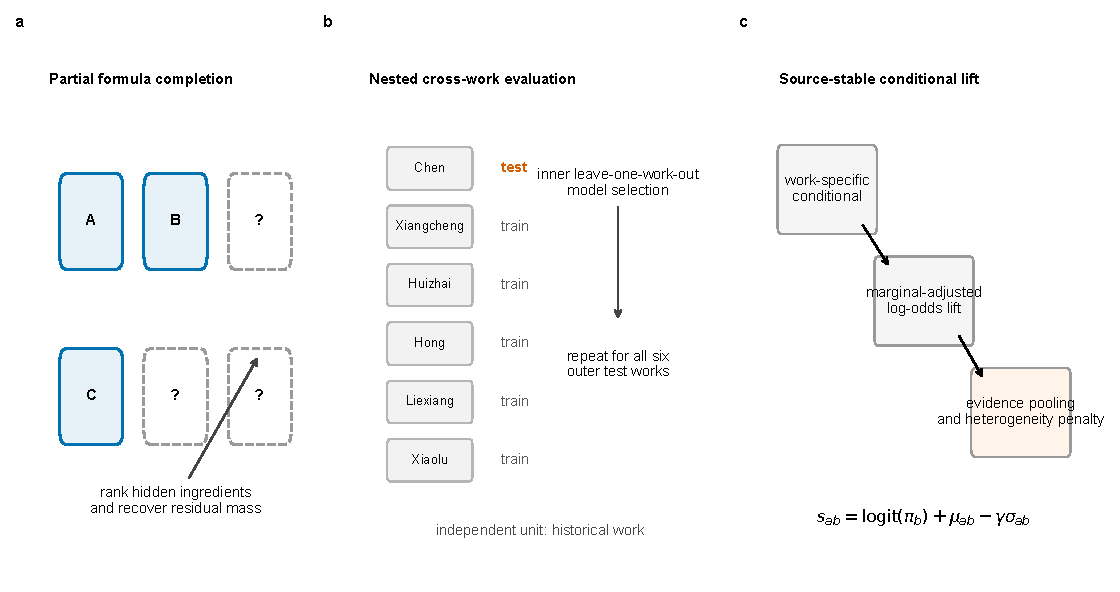
\includegraphics[width=\linewidth]{v2_fig1_design.pdf}
\caption{Model and evaluation design. \textbf{a}, The model receives an observed subset with fixed masses and ranks the hidden materials before allocating residual mass. \textbf{b}, Each outer fold excludes one historical work; hyperparameters are selected by inner leave-one-work-out evaluation on the remaining works. The procedure repeats for all six targets. \textbf{c}, \SSCL{} converts work-specific conditional probabilities to marginal-adjusted lifts, pools them by exposure, and subtracts a heterogeneity penalty. The primary task uses five deterministic masks at 50\% observed context.}
\label{fig:design}
\end{figure}

\subsection{Item models and graph diffusion}

EASE learns a dense linear item matrix \citep{steck2019ease}. With $P=(X^{\top}X+\rho I)^{-1}$,
\begin{equation}
B^{\mathrm{EASE}}_{ab}=
\begin{cases}
-P_{ab}/P_{bb}, & a\ne b,\\
0, & a=b.
\end{cases}
\label{eq:ease}
\end{equation}
The SLIM-style comparator fits each candidate column with a nonnegative elastic net \citep{ning2011slim}:
\begin{equation}
\widehat B=\arg\min_{B\ge0,\,\operatorname{diag}(B)=0}
\frac{1}{2N}\lVert X-XB\rVert_F^2+
\tau\left[\eta\lVert B\rVert_1+\frac{1-\eta}{2}\lVert B\rVert_F^2\right].
\label{eq:slim}
\end{equation}
For both models, the observed binary vector multiplies $B$, followed by a small prevalence tie-breaker. Personalized graph diffusion uses the row-normalized direct graph $T$ and restart vector $u_i$:
\begin{equation}
z_i^{(t+1)}=(1-\delta)u_i+\delta z_i^{(t)}T,
\qquad z_i^{(0)}=u_i.
\label{eq:ppr}
\end{equation}
Fifty iterations produce the PPR score. Formula k-nearest neighbours and PureSVD remain secondary comparators in the stricter two-work-held-out analysis.

\subsection{Ingredient count and composition}

All ranking models share one count rule. If $n_k$ is the number of training formulas with $k$ ingredients and $K_{\max}$ is the largest training count,
\begin{equation}
p_0(K=k)=\frac{n_k+\tfrac12}{N+K_{\max}/2},\qquad
p(K=k\mid o,f)\propto p_0(K=k)\mathbf{1}\{r(k,f)=o\}\mathbf{1}\{k\ge o+1\}.
\label{eq:count}
\end{equation}
The posterior median is $\widehat K_i$. The top-ranked hidden materials fill the remaining slots. This shared module makes count error identical across ranking methods.

Observed masses remain fixed. Let $m_i=1-\sum_{a\in O_i}w_{ia}$ be residual mass and $R_{ib}$ a nonnegative ratio score obtained from the ten most similar training formulas. For selected hidden set $\widehat H_i$,
\begin{equation}
\widehat w_{ib}=
\begin{cases}
w_{ib}, & b\in O_i,\\[2pt]
m_i R_{ib}/\sum_{h\in\widehat H_i}R_{ih}, & b\in\widehat H_i,\\[2pt]
0, & \text{otherwise}.
\end{cases}
\label{eq:composition}
\end{equation}

\subsection{Nested probability calibration}

The graph scores are treated as candidate probabilities only after calibration. For each outer test work, inner held-out-work predictions fit a temperature $T$ and a two-parameter logit map:
\begin{equation}
p^{(T)}=\sigma\!\left(\frac{\operatorname{logit}(p)}{T}\right),\qquad
p^{(L)}=\sigma\!\left(a\operatorname{logit}(p)+b\right),\quad a>0.
\label{eq:calibration}
\end{equation}
Parameters minimize candidate-level negative log likelihood inside the outer training data. The outer work contributes no calibration labels.

\section{Experimental Design}

\subsection{Nested cross-work protocol}

The primary analysis uses six outer leave-one-work-out folds. The target work is absent from vocabulary construction, prevalence estimates, graph edges, and hyperparameter selection. Inside each outer training set, leave-one-work-out validation selects the configuration with highest source-macro hidden F1, using weighted Jaccard as the tie-breaker. Five mask seeds are averaged first within formula, then within work. The six work means receive equal weight.

The model grids cover direct-graph smoothing $\alpha\in\{0.5,1,2,5\}$; \SSCL{} smoothing $\alpha\in\{1,2,5\}$, penalty $\gamma\in\{0,0.25,0.5,1\}$, blend $\lambda\in\{0.25,0.5,0.75,1\}$, and mean or maximum edge reduction. EASE ridge values range from 1 to 1000. SLIM tests four penalties and three $L_1$ ratios. PPR tests five diffusion values. Five of six outer folds selected a positive \SSCL{} heterogeneity penalty.

\subsection{Metrics and work-level inference}

Set recovery is measured on hidden ingredients only. For hidden truth $H_i$ and hidden prediction $\widehat H_i=\widehat S_i\mathbin{\backslash}O_i$,
\begin{align}
P_i&=\frac{|H_i\cap\widehat H_i|}{|\widehat H_i|},\qquad
R_i=\frac{|H_i\cap\widehat H_i|}{|H_i|},\qquad
F_{1i}=\frac{2P_iR_i}{P_i+R_i},\\
J_{wi}&=\frac{\sum_j\min(w_{ij},\widehat w_{ij})}
{\sum_j\max(w_{ij},\widehat w_{ij})}.
\label{eq:metrics}
\end{align}
Weighted Jaccard measures recovered composition mass. Count mean absolute error is \(|K_i-\widehat K_i|\).

For model $m$, the primary effect against frequency is the mean of paired work differences:
\begin{equation}
\widehat\Delta_m=\frac{1}{D}\sum_{d=1}^{D}
\left(\overline F_{1,md}-\overline F_{1,\mathrm{freq},d}\right),\qquad D=6.
\label{eq:estimand}
\end{equation}
An exact two-sided sign-flip test enumerates all $2^D$ work-level sign assignments:
\begin{equation}
p_{\mathrm{flip}}=2^{-D}\sum_{\vect{s}\in\{-1,1\}^{D}}
\mathbf{1}\!\left\{
\left|D^{-1}\sum_d s_d\Delta_{md}\right|\ge|\widehat\Delta_m|
\right\}.
\label{eq:signflip}
\end{equation}
The six blocks impose a coarse p-value grid. Formula masks are repeated measurements and are not treated as independent inferential units.

For calibration, Brier score and NLL are averaged first within formula and then within work. ACE is computed from candidate scores within each work. The final values are unweighted means across works. For labels $y_n\in\{0,1\}$ and probabilities $p_n$,
\begin{align}
\operatorname{Brier}&=L^{-1}\sum_{n=1}^{L}(p_n-y_n)^2,\\
\operatorname{NLL}&=-L^{-1}\sum_{n=1}^{L}\left[y_n\log p_n+(1-y_n)\log(1-p_n)\right],\\
\operatorname{ACE}&=\sum_{g=1}^{G}\frac{|I_g|}{L}
\left|\frac{1}{|I_g|}\sum_{n\in I_g}(p_n-y_n)\right|,
\label{eq:calmetrics}
\end{align}
where $I_g$ are equal-count groups within a work for ACE.

\subsection{Chemistry analysis}

The chemical registry links 18 of 81 materials to specimen-level analytical profiles from 17 publications and 40 PubChem compounds. Profiles retain taxon, plant part, preparation, analytical method, and measurement basis. Morgan fingerprints, physicochemical descriptors, and controlled odor tags form three similarities \citep{rogers2010_morgan}. The tested kernel is
\begin{equation}
K^{\mathrm{chem}}_{ab}=\omega_f T_{ab}+
\omega_x\max(0,C^{\mathrm{phys}}_{ab})+
\omega_o\max(0,C^{\mathrm{odor}}_{ab}),\qquad
\sum_r\omega_r=1.
\label{eq:chemkernel}
\end{equation}
Development ablation and a 44-formula inverse-odor task compare the kernel with a no-chemistry model and shuffled profile assignments. The ablation applies to the 18 covered materials and their recorded profiles.

\section{Results}

\subsection{Conditional relations transfer across work groups}

The directed graph reached source-macro hidden F1 0.426, compared with 0.378 for frequency (Table~\ref{tab:mainresults}). It improved five work groups and tied on Xiaolu. The mean paired difference was 0.0478, and the exact two-sided sign-flip p-value was 0.0625. \SSCL{} reached F1 0.4263, a difference of 0.0481 from frequency with the same five-positive, one-tie pattern and $p=0.0625$. EASE reached F1 0.4229 and the highest weighted Jaccard, 0.4730.

\SSCL{} and the direct graph produced nearly the same aggregate result. Their F1 difference was 0.0003, with paired $p=1.0$. The source-stability penalty therefore did not add measurable predictive value at this corpus size. The transferable gain came from conditioning on observed ingredients.

\begin{table}[t]
\centering
\caption{Nested six-work formula-completion performance at 50\% uniform observation. Values are unweighted means of work-level means. Count MAE is shared because every ranking model uses the same count module.}
\label{tab:mainresults}
\begin{threeparttable}
\begin{tabular}{lSSSSS}
\toprule
Model & {Precision} & {Recall} & {Hidden F1} & {Weighted Jaccard} & {Count MAE} \\
\midrule
Frequency & 0.4323 & 0.3633 & 0.3782 & 0.4514 & 1.1447 \\
Directed graph & 0.4808 & 0.4134 & 0.4260 & 0.4699 & 1.1447 \\
\SSCL{} & 0.4802 & 0.4138 & 0.4263 & 0.4716 & 1.1447 \\
EASE & 0.4793 & 0.4082 & 0.4229 & \bfseries 0.4730 & 1.1447 \\
SLIM & 0.4402 & 0.3713 & 0.3874 & 0.4545 & 1.1447 \\
PPR & 0.4672 & 0.3968 & 0.4119 & 0.4594 & 1.1447 \\
\bottomrule
\end{tabular}
\end{threeparttable}
\end{table}

\begin{figure}[t]
\centering
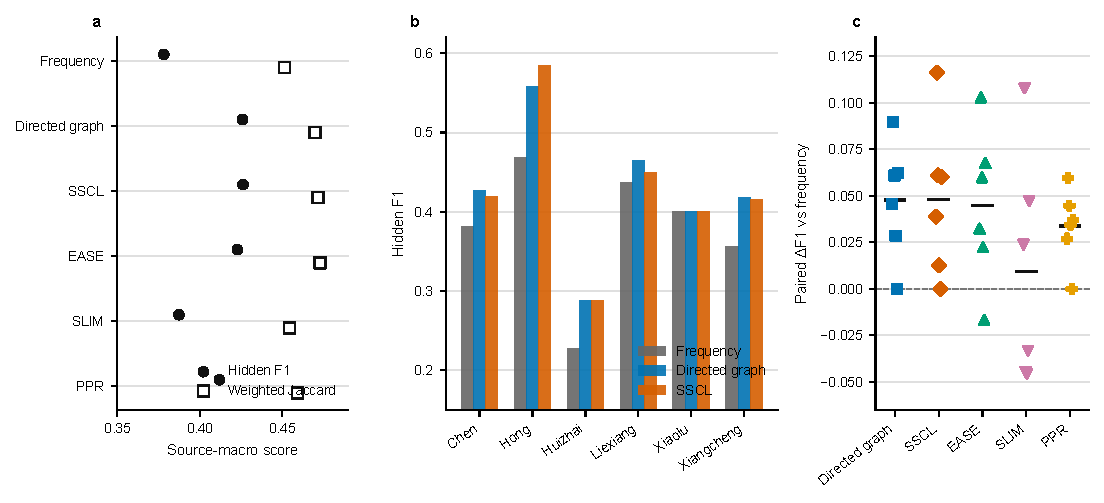
\includegraphics[width=\linewidth]{v2_fig2_performance.pdf}
\caption{Nested cross-work completion performance. \textbf{a}, Source-macro hidden F1 and weighted Jaccard for six models. \textbf{b}, Work-level hidden F1 for frequency, the directed graph, and \SSCL{}. Five deterministic masks are averaged within each of 90 evaluable formulas and then within each work. \textbf{c}, Paired work-level F1 differences from frequency; symbols are works and horizontal bars are means. For both graph and \SSCL{}, five works improve and one ties, giving an exact two-sided sign-flip $p=0.0625$. \SSCL{} differs from the directed graph by 0.0003 F1, $p=1.0$. Source data are provided with the figure.}
\label{fig:performance}
\end{figure}

The work-level range was substantial (Table~\ref{tab:workresults}). Hong reached the highest graph scores, whereas Huizhai remained below 0.29 for every structured model. The Xiaolu estimate is based on two formulas and yields a tie among frequency, graph, and \SSCL{}. Equal work weighting keeps the large Chen and Xiangcheng groups from determining the full result.

\begin{table}[t]
\centering
\caption{Hidden F1 by held-out work. The row count gives evaluable formulas; each formula score averages five masks.}
\label{tab:workresults}
\begin{tabular}{lrrrrr}
\toprule
Work & $n$ & Frequency & Directed graph & \SSCL{} & EASE \\
\midrule
Chen & 38 & 0.3812 & 0.4268 & 0.4199 & 0.4135 \\
Hong & 6 & 0.4689 & 0.5583 & 0.5850 & 0.5717 \\
Huizhai & 9 & 0.2268 & 0.2877 & 0.2877 & 0.2867 \\
Liexiang & 6 & 0.4365 & 0.4649 & 0.4490 & 0.4588 \\
Xiaolu & 2 & 0.4000 & 0.4000 & 0.4000 & 0.3833 \\
Xiangcheng & 29 & 0.3557 & 0.4180 & 0.4159 & 0.4232 \\
\bottomrule
\end{tabular}
\end{table}

\subsection{A stricter two-work-held-out test preserves the scale of the gain}

A secondary protocol used five development work groups, selected configurations by leave-one-work-out validation, and evaluated all ten pairs of held-out works. The direct graph reached hidden F1 0.3672 versus 0.3386 for frequency (Table~\ref{tab:hardshift}). Formula k-nearest neighbours reached 0.3431 and PureSVD 0.3343. \SSCL{} reached 0.3650 and again did not exceed the direct graph. Weighted Jaccard favored the direct graph among V2 models and formula k-nearest neighbours across all listed comparators.

\begin{table}[t]
\centering
\caption{Secondary two-work-held-out source-shift evaluation at 50\% uniform observation.}
\label{tab:hardshift}
\begin{tabular}{lSSSS}
\toprule
Model & {Precision} & {Recall} & {Hidden F1} & {Weighted Jaccard} \\
\midrule
Frequency & 0.4054 & 0.3160 & 0.3386 & 0.4400 \\
Formula kNN & 0.4082 & 0.3233 & 0.3431 & 0.4435 \\
PureSVD & 0.3948 & 0.3161 & 0.3343 & 0.4200 \\
Directed graph & 0.4368 & 0.3437 & \bfseries 0.3672 & \bfseries 0.4494 \\
\SSCL{} & 0.4303 & 0.3451 & 0.3650 & 0.4423 \\
EASE & 0.4315 & 0.3398 & 0.3625 & 0.4450 \\
SLIM & 0.3831 & 0.3122 & 0.3273 & 0.4408 \\
PPR & 0.4315 & 0.3384 & 0.3618 & 0.4445 \\
\bottomrule
\end{tabular}
\end{table}

\subsection{Missingness mechanism changes model ordering}

At the primary 50\% context, all structured models exceeded frequency under all four observation mechanisms (Table~\ref{tab:missingness}). Their ordering changed. The directed graph led abundance-biased retention at F1 0.4295. EASE led prefix retention at 0.4812. \SSCL{} led the unknown-fraction task at 0.4038. At 75\% prefix retention, \SSCL{} reached 0.4619, compared with 0.3951 for frequency. At 75\% abundance-biased retention, frequency reached 0.3550 and exceeded the structured models.

Hidden F1 does not rise monotonically with observed fraction because the target set changes. A larger observed subset leaves fewer hidden ingredients and can concentrate rare materials in the residual task. The uniform and unknown-fraction panels show this decline clearly.

\begin{table}[t]
\centering
\caption{Source-macro hidden F1 under four observation mechanisms at 50\% observed context.}
\label{tab:missingness}
\begin{tabular}{lrrrr}
\toprule
Mechanism & Frequency & Directed graph & \SSCL{} & EASE \\
\midrule
Uniform & 0.3782 & 0.4260 & \bfseries 0.4263 & 0.4229 \\
Abundance-biased & 0.3885 & \bfseries 0.4295 & 0.4255 & 0.4288 \\
Source-list prefix & 0.3986 & 0.4681 & 0.4662 & \bfseries 0.4812 \\
Unknown fraction & 0.3781 & 0.3920 & \bfseries 0.4038 & 0.3868 \\
\bottomrule
\end{tabular}
\end{table}

\begin{figure}[t]
\centering
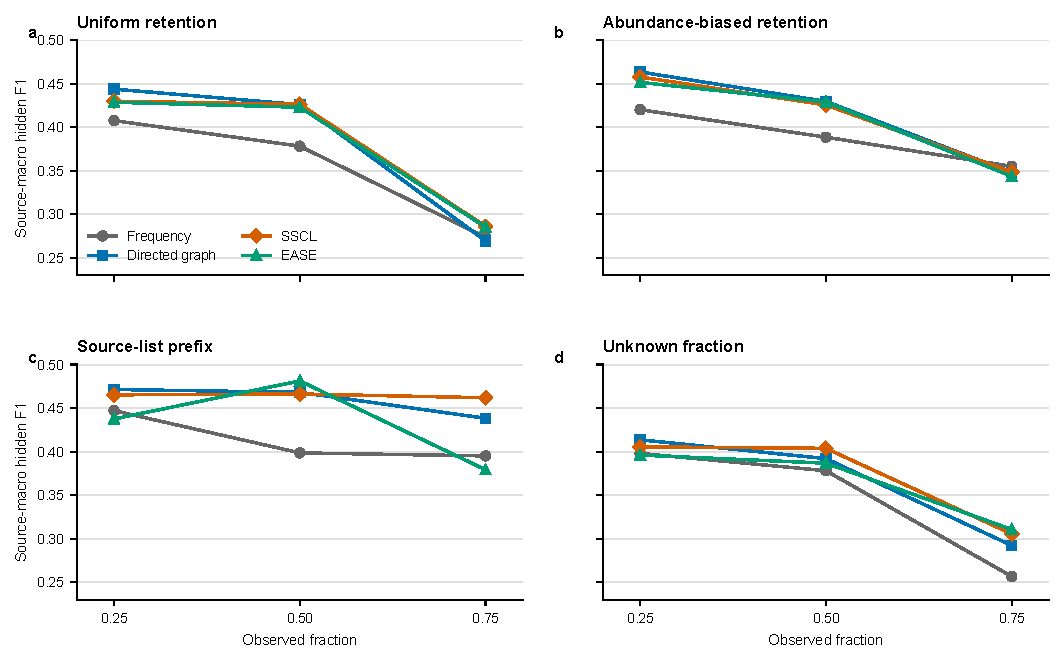
\includegraphics[width=\linewidth]{v2_fig3_missingness.pdf}
\caption{Sensitivity to the observation mechanism. \textbf{a}, Uniform ingredient retention. \textbf{b}, Retention weighted by reference mass. \textbf{c}, Retention of the first ingredients in source order. \textbf{d}, Uniform retention with an unknown observed fraction in the count decoder. Points are source-macro means across six outer work folds; five deterministic masks are averaged within formula and work. Shared axes expose changes in both absolute difficulty and model ordering. Source data are provided with the figure.}
\label{fig:missingness}
\end{figure}

\subsection{Nested logit calibration removes unsupported high scores}

The uncalibrated \SSCL{} scores had source-macro Brier 0.0427, NLL 0.1572, and ACE 0.0579 (Table~\ref{tab:calibration}). Temperature scaling reduced each error. The two-parameter logit map produced Brier 0.0340, NLL 0.1262, and ACE 0.0145. Each outer calibrator was fitted exclusively on inner held-out-work predictions.

Before calibration, 186 candidate scores exceeded 0.8; their mean score was 0.839 and empirical inclusion frequency was 0.608. Logit calibration left two scores above 0.8, too few for a stable high-bin estimate. The recalibrated distribution also produced lower work-macro errors.

\begin{table}[t]
\centering
\caption{Nested calibration of \SSCL{} candidate scores. Lower Brier, NLL, and ACE values are better. The final three columns describe predictions with $p>0.8$.}
\label{tab:calibration}
\begin{tabular}{lrrrrrr}
\toprule
Method & Brier & NLL & ACE & Count & Mean $p$ & Empirical frequency \\
\midrule
Uncalibrated & 0.0427 & 0.1572 & 0.0579 & 186 & 0.839 & 0.608 \\
Temperature & 0.0406 & 0.1456 & 0.0371 & 455 & 0.874 & 0.527 \\
Logit & \bfseries 0.0340 & \bfseries 0.1262 & \bfseries 0.0145 & 2 & 0.831 & 1.000 \\
\bottomrule
\end{tabular}
\end{table}

\begin{figure}[t]
\centering
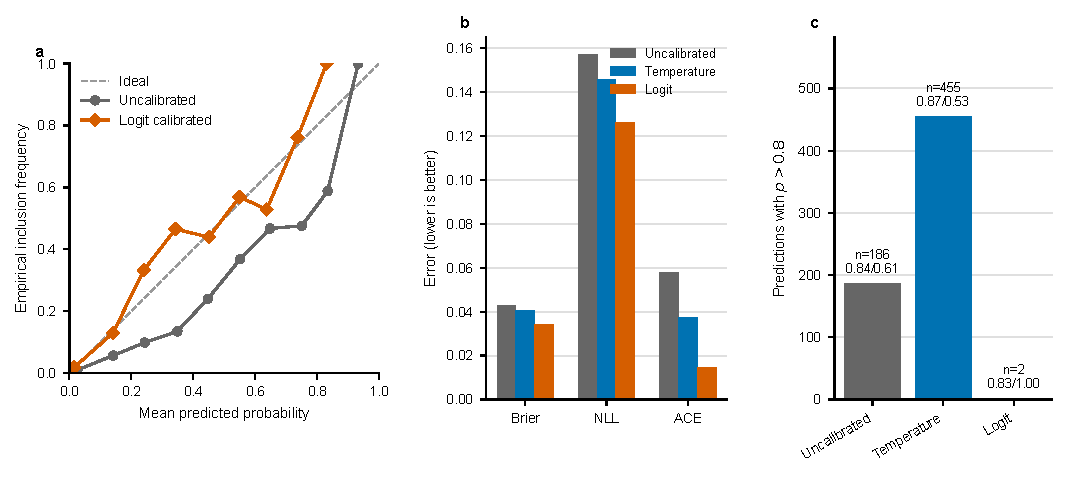
\includegraphics[width=\linewidth]{v2_fig4_calibration.pdf}
\caption{Nested probability calibration. \textbf{a}, Pooled reliability bins before and after logit calibration; bin counts are available in source data. \textbf{b}, Source-macro Brier score, negative log likelihood, and adaptive calibration error. \textbf{c}, Number of predictions above 0.8; labels give count followed by mean probability and empirical inclusion frequency. Calibrators are fitted to inner held-out-work predictions for each outer fold. Only two logit-calibrated predictions remain above 0.8, so their empirical frequency is descriptive. Source data are provided with the figure.}
\label{fig:calibration}
\end{figure}

\subsection{The current chemistry kernel adds no completion gain}

The best chemistry-enabled development variant reached hidden F1 0.3905, compared with 0.3911 for its non-chemistry counterpart. In the 44-formula inverse-odor analysis, odor kNN reached weighted Jaccard 0.2913. The forward-consistent model reached 0.2824, its no-chemistry ablation 0.2835, and shuffled chemical profiles 0.2863. These results identify no benefit from the current pairwise similarity kernel. The analysis covers 18 materials and does not test combustion products, concentration-dependent perception, or mixture suppression.

\section{Discussion}

The benchmark gives a consistent answer to the central question. Conditional ingredient relations transfer across historical work groups and raise hidden-ingredient F1 by about 0.048 over global frequency in nested six-work evaluation. The same scale appears in the stricter two-work-held-out protocol. EASE and PPR also improve on frequency, so the evidence supports a general graph and item-dependency interpretation.

Source heterogeneity matters to evaluation more than to the present predictor. Five outer folds selected a positive dispersion penalty, yet \SSCL{} and the direct graph differed by 0.0003 F1. The corpus supplies only five training work groups in each outer fold, and several materials appear in a single formula. Under those conditions, source-specific edge variance is noisy and shrinkage dominates. More independently curated works would let the heterogeneity term distinguish stable relations from compilation-specific ones.

The missingness experiments change the practical interpretation of a completion score. Prefix retention preserves editorial order and produced higher F1 for graph models at large observed fractions. Abundance-biased retention favored common high-mass ingredients in the context and changed the residual set enough for frequency to lead at $f=0.75$. A benchmark that reports only uniform random masking gives one answer to a family of observation processes.

The chemistry analysis defines the next modeling problem. Pairwise chemical resemblance can encode substitution, whereas incense formulas can pair dissimilar materials for volatility, contrast, binding, or combustion behavior. A chemistry-aware extension should represent directed roles and mixture interactions. Useful variables include volatile class, boiling-point distribution, odor threshold, pyrolysis products, and preparation state. Those features require formula-linked measurements or a substantially broader evidence registry.

Probability calibration has an immediate operational effect. The raw graph produced many high scores whose empirical inclusion rate was much lower. Nested logit calibration shifted them into probability regions supported by held-out works and improved all three work-macro error measures. Ranked completions can therefore be accompanied by probabilities without treating the graph score itself as calibrated evidence.

\section{Limitations}

The independent sample consists of six work groups, and two groups contain six formulas or fewer. Exact work-level inference consequently has low resolution. The corpus was canonicalized by one curator, so it has no inter-annotator agreement estimate. Source genealogy can also create dependence between work groups even after retaining one representative per provisional formula family.

The prediction task starts from known ingredients. It does not infer a recipe from a title or literary odor description alone. Relative historical quantities support compositional comparison, but they do not reproduce processing loss, burning temperature, headspace concentration, or sensory perception. The chemical registry covers 18 materials and cannot support a general conclusion about chemical predictors. Finally, the observation mechanisms are controlled simulations of textual loss; a larger collection of genuinely damaged or variant manuscripts is needed to estimate historical missingness directly.

\section{Conclusion}

Historical incense formula recovery can be evaluated as source-shifted weighted set completion. Across six held-out work groups, conditional co-formulation raised hidden-ingredient F1 from 0.378 to about 0.426. The proposed source-stability penalty matched the direct graph and did not improve it. Missingness mechanism altered model ordering, and nested logit calibration substantially improved candidate probabilities. These findings set a reproducible baseline for future work that adds independent texts, replicated annotation, formula-linked chemistry, and real transmission variants.

\section*{Data and Code Availability}

The repository contains the curated formula records, source locators, material ontology, deterministic split definitions, experiment configurations, model code, tests, figure source data, and scripts used to generate every reported result. Public release should preserve source attribution and the rights statements stored with each record.

\section*{Ethics Statement}

The study analyzes public historical texts and published chemical records. It contains no human participants, personal data, or animal experiments.

\bibliographystyle{unsrtnat}
\bibliography{xiangji_cgir_references,xiangji_cgir_v2_methods}

\end{document}
